\documentclass[
  degree=mecinf,
  title=normal,
  toc=normal,
  bib=normal]{mnye}

\usepackage{booktabs}
\usepackage{ebox}
\usepackage{enotation}
\usepackage{emargintag}
\usepackage{emedia}

\providecommand{\tightlist}{%
  \setlength{\itemsep}{0pt}\setlength{\parskip}{0pt}}


% preamble


\addbibresource{book.bib}
\addbibresource{packages.bib}

\usepackage{color}
\usepackage{fancyvrb}
\newcommand{\VerbBar}{|}
\newcommand{\VERB}{\Verb[commandchars=\\\{\}]}
\DefineVerbatimEnvironment{Highlighting}{Verbatim}{commandchars=\\\{\}}
% Add ',fontsize=\small' for more characters per line
\usepackage{framed}
\definecolor{shadecolor}{RGB}{248,248,248}
\newenvironment{Shaded}{\begin{snugshade}}{\end{snugshade}}
\newcommand{\AlertTok}[1]{\textcolor[rgb]{0.94,0.16,0.16}{#1}}
\newcommand{\AnnotationTok}[1]{\textcolor[rgb]{0.56,0.35,0.01}{\textbf{\textit{#1}}}}
\newcommand{\AttributeTok}[1]{\textcolor[rgb]{0.77,0.63,0.00}{#1}}
\newcommand{\BaseNTok}[1]{\textcolor[rgb]{0.00,0.00,0.81}{#1}}
\newcommand{\BuiltInTok}[1]{#1}
\newcommand{\CharTok}[1]{\textcolor[rgb]{0.31,0.60,0.02}{#1}}
\newcommand{\CommentTok}[1]{\textcolor[rgb]{0.56,0.35,0.01}{\textit{#1}}}
\newcommand{\CommentVarTok}[1]{\textcolor[rgb]{0.56,0.35,0.01}{\textbf{\textit{#1}}}}
\newcommand{\ConstantTok}[1]{\textcolor[rgb]{0.00,0.00,0.00}{#1}}
\newcommand{\ControlFlowTok}[1]{\textcolor[rgb]{0.13,0.29,0.53}{\textbf{#1}}}
\newcommand{\DataTypeTok}[1]{\textcolor[rgb]{0.13,0.29,0.53}{#1}}
\newcommand{\DecValTok}[1]{\textcolor[rgb]{0.00,0.00,0.81}{#1}}
\newcommand{\DocumentationTok}[1]{\textcolor[rgb]{0.56,0.35,0.01}{\textbf{\textit{#1}}}}
\newcommand{\ErrorTok}[1]{\textcolor[rgb]{0.64,0.00,0.00}{\textbf{#1}}}
\newcommand{\ExtensionTok}[1]{#1}
\newcommand{\FloatTok}[1]{\textcolor[rgb]{0.00,0.00,0.81}{#1}}
\newcommand{\FunctionTok}[1]{\textcolor[rgb]{0.00,0.00,0.00}{#1}}
\newcommand{\ImportTok}[1]{#1}
\newcommand{\InformationTok}[1]{\textcolor[rgb]{0.56,0.35,0.01}{\textbf{\textit{#1}}}}
\newcommand{\KeywordTok}[1]{\textcolor[rgb]{0.13,0.29,0.53}{\textbf{#1}}}
\newcommand{\NormalTok}[1]{#1}
\newcommand{\OperatorTok}[1]{\textcolor[rgb]{0.81,0.36,0.00}{\textbf{#1}}}
\newcommand{\OtherTok}[1]{\textcolor[rgb]{0.56,0.35,0.01}{#1}}
\newcommand{\PreprocessorTok}[1]{\textcolor[rgb]{0.56,0.35,0.01}{\textit{#1}}}
\newcommand{\RegionMarkerTok}[1]{#1}
\newcommand{\SpecialCharTok}[1]{\textcolor[rgb]{0.00,0.00,0.00}{#1}}
\newcommand{\SpecialStringTok}[1]{\textcolor[rgb]{0.31,0.60,0.02}{#1}}
\newcommand{\StringTok}[1]{\textcolor[rgb]{0.31,0.60,0.02}{#1}}
\newcommand{\VariableTok}[1]{\textcolor[rgb]{0.00,0.00,0.00}{#1}}
\newcommand{\VerbatimStringTok}[1]{\textcolor[rgb]{0.31,0.60,0.02}{#1}}
\newcommand{\WarningTok}[1]{\textcolor[rgb]{0.56,0.35,0.01}{\textbf{\textit{#1}}}}




\title{Ajuste de datos con R}

\term{2020-2021}

\begin{document}

% Before Body

\hypertarget{introducciuxf3n}{%
\section*{Introducción}\label{introducciuxf3n}}

En esta práctica estudiaremos cómo ajustar un modelo a un conjunto de datos experimentales, mediante la técnica de mínimos cuadrados, usando \textsf{R}.

Mientras que en los problemas que hemos a mano hasta ahora hemos considerado únicamente modelos lineales de uno o dos parámetros, en esta práctica consideraremos modelos tanto lineales como no lineales, y con un número arbitrario de parámetros.

Seguiremos trabajando con una variable dependiente \(y\) y una única variable dependiente \(x\), aunque las técnicas que presentaremos se generalizan sin dificultad al caso de varias variables independientes.

\hypertarget{requisitos-previos}{%
\section{Requisitos previos}\label{requisitos-previos}}

Antes de comenzar esta práctica, necesitas:

\begin{itemize}
\item
  Tener \textsf{R} y \textsf{RStudio} instalados en tu equipo. Ver \href{https://emazcunan.github.io/install-r-rstudio/}{Instalación de R y RStudio}
\item
  Haber estudiado la práctica \href{https://emazcunan.github.io/basics-r-rstudio/}{Primeros pasos con R y RStudio}
\end{itemize}

Para utilizar las funciones que aparecerán a lo largo de la prácticam empezamos cargando el paquete tidyverse:

\begin{Shaded}
\begin{Highlighting}[]
\FunctionTok{library}\NormalTok{(}\StringTok{"tidyverse"}\NormalTok{)}
\end{Highlighting}
\end{Shaded}

\hypertarget{lm}{%
\section{Modelos lineales}\label{lm}}

Como hemos visto en teoría, dada una variable dependiente \(y\) y una variable independiente \(x\), un modelo lineal de parámetros \(\beta_1\), \(\beta_2\), \ldots{} \(\beta_p\) tiene la forma

\[
y = \beta_1 f_1(x) + \beta_2 f_2(x) + \dots +\beta_p f_p(x),
\]
siendo \(f_1\), \(f_2\), \(\dots\), \(f_p\) funciones conocidas.

En este capítulo veremos cómo ajustar este tipo de modelos a las observaciones recogidas en una hoja de datos, usando la función \texttt{lm()} (\textbf{l}inear \textbf{m}odel) de \textsf{R}.

Veremos también cómo representar gráficamente un ajuste usando la función \texttt{geom\_smooth()} del paquete \texttt{ggplot2}.

\hypertarget{planteamiento-del-problema-el-prisma-de-vidrio}{%
\subsection{Planteamiento del problema: El prisma de vidrio}\label{planteamiento-del-problema-el-prisma-de-vidrio}}

Newton demostró con el prisma que la luz blanca es una mezcla de varios colores y que la refracción depende del color (longitud de onda).

En un experimento, se eligieron diferentes longitudes de onda \(\lambda\) y se trazó el camino seguido por el rayo de luz que atraviesa el prisma, midiendo el ángulo de desviación para a partir del mismo calcular el índice de refracción \(n\) del vidrio para el color seleccionado. Los datos obtenidos se recogen en el archivo \href{https://drive.google.com/uc?export=download\&id=1fI5_KZA8MAiZVegFmtlQ7Cm4IzlGDQtg}{\texttt{cauchy.csv}}(click para descargar), que contiene las variables:

\begin{itemize}
\item
  \texttt{lambda}: longitud de onda \(\lambda\), medida en \(nm\).
\item
  \texttt{n}: índice de refracción.
\end{itemize}

Descarga el fichero \texttt{cauchy.csv} y guárdalo en una carpeta de nombre \texttt{data} dentro de tu directorio de trabajo.

Importamos los datos con \texttt{read\_csv()} y los guardamos en un objeto de nombre \texttt{cauchy}:

\begin{Shaded}
\begin{Highlighting}[]
\NormalTok{cauchy }\OtherTok{\textless{}{-}} \FunctionTok{read\_csv}\NormalTok{(}\StringTok{"data/cauchy.csv"}\NormalTok{)}
\end{Highlighting}
\end{Shaded}

Visualizamos los datos dibujando la nube de puntos \((\lambda, n)\) con \texttt{geom\_point()}:

\begin{Shaded}
\begin{Highlighting}[]
\FunctionTok{ggplot}\NormalTok{(}
    \AttributeTok{data =}\NormalTok{ cauchy,}
    \AttributeTok{mapping =} \FunctionTok{aes}\NormalTok{(}\AttributeTok{x =}\NormalTok{ lambda, }\AttributeTok{y =}\NormalTok{ n)}
\NormalTok{) }\SpecialCharTok{+} 
    \FunctionTok{geom\_point}\NormalTok{()}
\end{Highlighting}
\end{Shaded}

\begin{center}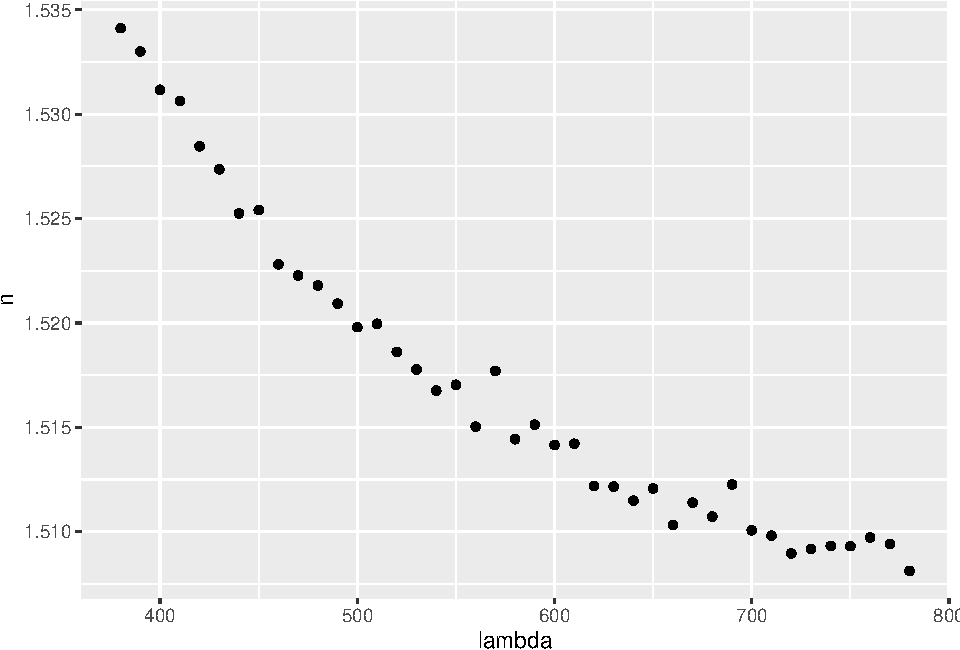
\includegraphics[width=1\linewidth]{Pr1-fitting_files/figure-latex/unnamed-chunk-5-1} \end{center}

\hypertarget{ajuste-con-lm}{%
\subsection{\texorpdfstring{Ajuste con \texttt{lm()}}{Ajuste con lm()}}\label{ajuste-con-lm}}

Tomaremos como modelo la fórmula de Cauchy para los índices de refracción \(n\) en la región visible del espectro de longitud de onda \(\lambda\):
\[n(\lambda) = \beta_1 + \frac{\beta_2}{\lambda^2} + \frac{\beta_3}{\lambda^4}\]
donde \(\beta_1\), \(\beta_2\) y \(\beta_3\) son los parámetros a ajustar.

Como se indicó antes, la función de \textsf{R} para ajustar modelos lineales es \texttt{lm()}.

\begin{Shaded}
\begin{Highlighting}[]
\NormalTok{fit\_cauchy }\OtherTok{\textless{}{-}} \FunctionTok{lm}\NormalTok{(}
        \AttributeTok{data =}\NormalTok{ cauchy, }
        \AttributeTok{formula =}\NormalTok{ n }\SpecialCharTok{\textasciitilde{}} \FunctionTok{I}\NormalTok{(}\DecValTok{1}\SpecialCharTok{/}\NormalTok{lambda}\SpecialCharTok{\^{}}\DecValTok{2}\NormalTok{) }\SpecialCharTok{+} \FunctionTok{I}\NormalTok{(}\DecValTok{1}\SpecialCharTok{/}\NormalTok{lambda}\SpecialCharTok{\^{}}\DecValTok{4}\NormalTok{)}
\NormalTok{    )}
\end{Highlighting}
\end{Shaded}

En el código anterior, se utiliza la función \texttt{lm()} para ajustar el modelo propuesto a las observaciones de nuestra hoja de datos.
Hemos usado los argumentos \texttt{data}, para especificar la hoja de datos con las observaciones, y \texttt{formula}, para indicar la fórmula del modelo (enseguida explicaremos cómo construir esta fórmula).

El resultado se almacena en un objeto de nombre \texttt{fit\_cauchy}.

Si imprimimos el objeto \texttt{fit\_cauchy} veremos los coeficientes del ajuste:

\begin{Shaded}
\begin{Highlighting}[]
\NormalTok{fit\_cauchy}
\end{Highlighting}
\end{Shaded}

\begin{verbatim}
## 
## Call:
## lm(formula = n ~ I(1/lambda^2) + I(1/lambda^4), data = cauchy)
## 
## Coefficients:
##   (Intercept)  I(1/lambda^2)  I(1/lambda^4)  
##           1.5         4908.3      7078041.7
\end{verbatim}

Pero la instrucción \texttt{summary(fit\_cauchy)} revela que el objeto contiene mucha más información de la que muestra su simple impresión:

\begin{Shaded}
\begin{Highlighting}[]
\FunctionTok{summary}\NormalTok{(fit\_cauchy)}
\end{Highlighting}
\end{Shaded}

\begin{verbatim}
## 
## Call:
## lm(formula = n ~ I(1/lambda^2) + I(1/lambda^4), data = cauchy)
## 
## Residuals:
##        Min         1Q     Median         3Q        Max 
## -1.294e-03 -4.672e-04  1.711e-05  2.982e-04  2.216e-03 
## 
## Coefficients:
##                Estimate Std. Error  t value Pr(>|t|)    
## (Intercept)   1.500e+00  7.676e-04 1954.496  < 2e-16 ***
## I(1/lambda^2) 4.908e+03  4.342e+02   11.303 1.02e-13 ***
## I(1/lambda^4) 7.078e+06  5.376e+07    0.132    0.896    
## ---
## Signif. codes:  0 '***' 0.001 '**' 0.01 '*' 0.05 '.' 0.1 ' ' 1
## 
## Residual standard error: 0.0007213 on 38 degrees of freedom
## Multiple R-squared:  0.9912, Adjusted R-squared:  0.9907 
## F-statistic:  2131 on 2 and 38 DF,  p-value: < 2.2e-16
\end{verbatim}

Ésta es la razón por la que hemos creado el objeto \texttt{fit\_cauchy} para almacenar el resultado de la función \texttt{lm()}: lo usaremos en los siguientes apartados para extraer información del ajuste realizado.

\hypertarget{fuxf3rmulas-en-r}{%
\subsection{Fórmulas en R}\label{fuxf3rmulas-en-r}}

Al usar la función \texttt{lm()}, hemos indicado el siguiente valor para el argumento \texttt{formula} :

\texttt{n\ \textasciitilde{}\ I(1/lambda\^{}2)\ +\ I(1/lambda\^{}4)}

La expresión anterior es un objeto de \textsf{R} de tipo \texttt{formula}, que se corresponde con la fórmula del módelo

\[n = \beta_1 + \frac{\beta_2}{\lambda^2} + \frac{\beta_3}{\lambda^4}.\]

En la siguiente tabla se muestran algunos ejemplos más de fórmulas en \textsf{R} correspondientes a diferentes modelos:

\begin{longtable}[]{@{}cc@{}}
\toprule
Modelo & \texttt{formula} \\
\midrule
\endhead
\(y=\beta_1+\beta_2x\) & \texttt{y\ \textasciitilde{}\ x} \\
\(y=\beta_1 x\) & \texttt{y\ \textasciitilde{}\ 0\ +\ x} \\
\(y=\beta_1 + \beta_2 x + \beta_3 x^2\) & \texttt{y\ \textasciitilde{}\ x\ +\ I(x\^{}2)} \\
\(y=\beta_1 \cos(x)+ \beta_2\sin(x)\) & \texttt{y\ \textasciitilde{}\ 0\ +\ I(cos(x))\ +\ I(sin(x))} \\
\bottomrule
\end{longtable}

Para especificar la fórmula de un modelo en \textsf{R} hay que tener en cuenta las siguientes reglas:

\begin{itemize}
\item
  Cada sumando en una fórmula de \textsf{R}, indica la función que multiplica a un parámetro em la fórmula del modelo. Así, el sumando \texttt{x} en una fórmula de \textsf{R} será un sumando de la forma \(\beta_ix\) en la fórmula matemática del modelo.
\item
  \textsf{R} añade siempre una constante como primer sumando de la fórmula del modelo (\(\beta_1\) en los ejemplos anteriores). Para evitar la inclusión automática de esa constante, hay que escribir el sumando \texttt{0}. Así, la fórmula \texttt{y\ \textasciitilde{}\ x} se corresponde con \(y = \beta_1 + \beta_2x\); y si se quiere omitir la constante \texttt{\textbackslash{}beta\_1}, se ha de escribir \texttt{y\ \textasciitilde{}\ 0\ +\ x}.
\item
  Las funciones que son una transformación de la variable independiente se han de escribir incluidas en la función \texttt{I()}. Por ejemplo, un término de la forma \(\beta_i x^2\) en la fórmula de un modelo se escribe en \textsf{R} como \texttt{I(x\^{}2)}.
\end{itemize}

\hypertarget{coeficientes}{%
\subsection{Coeficientes}\label{coeficientes}}

Para obtener los coeficientes del ajuste usamos las función \texttt{coefficients()}:

\begin{Shaded}
\begin{Highlighting}[]
\FunctionTok{coefficients}\NormalTok{(fit\_cauchy) }
\end{Highlighting}
\end{Shaded}

\begin{verbatim}
##   (Intercept) I(1/lambda^2) I(1/lambda^4) 
##  1.500310e+00  4.908268e+03  7.078042e+06
\end{verbatim}

La salida nos informa de que los coeficientes que solucionan el problema de mínimos cuadrados (ecuaciones normales de Gauss) son:
\[\hat{\beta_1} = 1.50031,\]
\[\hat{\beta_2} = 4908.268,\]
y
\[\hat{\beta_3} = 7078042.\]

\textbf{Nota:} Dependiendo de la configuración, los valores de la salida pueden aparecer en notación científica, simbolizando \texttt{e+00}, \texttt{e+03} y \texttt{e+06} que hay que multiplicar por \(10^0=1\), \(10^3=1000\) y \(10^6=1000000\) respectivamente.

Por tanto el ajuste buscado es
\[n = 1.50031 + \frac{4908.268}{\lambda^2} + \frac{7078042}{\lambda^4}.\]

\hypertarget{valores-ajustados}{%
\subsection{Valores ajustados}\label{valores-ajustados}}

Los valores ajustados (o esperados) para la variable dependiente se obtienen con la función \texttt{fitted()}:

\begin{Shaded}
\begin{Highlighting}[]
\FunctionTok{fitted}\NormalTok{(fit\_cauchy)}
\end{Highlighting}
\end{Shaded}

\begin{verbatim}
##        1        2        3        4        5        6        7        8 
## 1.534640 1.532886 1.531263 1.529759 1.528362 1.527062 1.525851 1.524721 
##        9       10       11       12       13       14       15       16 
## 1.523664 1.522674 1.521746 1.520875 1.520056 1.519285 1.518558 1.517873 
##       17       18       19       20       21       22       23       24 
## 1.517225 1.516613 1.516033 1.515484 1.514963 1.514468 1.513998 1.513552 
##       25       26       27       28       29       30       31       32 
## 1.513126 1.512721 1.512335 1.511967 1.511615 1.511279 1.510958 1.510650 
##       33       34       35       36       37       38       39       40 
## 1.510356 1.510074 1.509804 1.509545 1.509297 1.509058 1.508829 1.508608 
##       41 
## 1.508396
\end{verbatim}

\hypertarget{residuos}{%
\subsection{Residuos}\label{residuos}}

Para obtener los residuos del ajuste usamos la función \texttt{residuals()}:

\begin{Shaded}
\begin{Highlighting}[]
\FunctionTok{residuals}\NormalTok{(fit\_cauchy)}
\end{Highlighting}
\end{Shaded}

\begin{verbatim}
##             1             2             3             4             5 
## -5.158258e-04  1.192086e-04 -9.157603e-05  8.724810e-04  9.998852e-05 
##             6             7             8             9            10 
##  2.981569e-04 -6.063847e-04  6.853349e-04 -8.594240e-04 -3.992586e-04 
##            11            12            13            14            15 
##  4.507231e-05  4.592263e-05 -2.575917e-04  6.782515e-04  5.616847e-05 
##            16            17            18            19            20 
## -1.021129e-04 -4.671765e-04  4.270844e-04 -1.002945e-03  2.215907e-03 
##            21            22            23            24            25 
## -5.376294e-04  6.594862e-04  1.524706e-04  6.591191e-04 -9.333365e-04 
##            26            27            28            29            30 
## -5.619564e-04 -8.481528e-04  9.871010e-05 -1.294146e-03  1.065956e-04 
##            31            32            33            34            35 
## -2.355407e-04  1.609116e-03 -2.899098e-04 -2.667854e-04 -8.491117e-04 
##            36            37            38            39            40 
## -3.842938e-04  1.710620e-05  2.483173e-04  8.932864e-04  7.950677e-04 
##            41 
## -2.796932e-04
\end{verbatim}

Para calcular el error cuadrático del ajuste (\(RSS\)) usamos

\begin{Shaded}
\begin{Highlighting}[]
\FunctionTok{sum}\NormalTok{(}\FunctionTok{residuals}\NormalTok{(fit\_cauchy)}\SpecialCharTok{\^{}}\DecValTok{2}\NormalTok{)}
\end{Highlighting}
\end{Shaded}

\begin{verbatim}
## [1] 1.976785e-05
\end{verbatim}

En el resumen del ajuste podemos leer

\texttt{Residual\ standard\ error:\ 0.0007213\ on\ 38\ degrees\ of\ freedom}

El error estandard residual, que suele denotarse \(\sigma\), se obtiene con la función \texttt{sigma()}. La relación entre esta cantidad \(\sigma\) y el error cuadrático \(RSS\) es:
\[\sigma = \sqrt{RSS/38}\]
o equivalentemente
\[RSS=38\sigma^2.\]
El valor \(38\), se llama grados de libertad de los residuos y se obtiene de restar, a las \(n=41\) observaciones, los \(p=3\) parámetros del modelo. Se obtiene con la función \texttt{df.residual()}.

\begin{Shaded}
\begin{Highlighting}[]
\FunctionTok{sigma}\NormalTok{(fit\_cauchy)}
\FunctionTok{df.residual}\NormalTok{(fit\_cauchy)}\SpecialCharTok{*}\FunctionTok{sigma}\NormalTok{(fit\_cauchy)}\SpecialCharTok{\^{}}\DecValTok{2} \CommentTok{\# RSS}
\end{Highlighting}
\end{Shaded}

\begin{verbatim}
## [1] 0.0007212534
## [1] 1.976785e-05
\end{verbatim}

\hypertarget{predicciones}{%
\subsection{Predicciones}\label{predicciones}}

La siguiente tabla recoge las longitudes de onda correspondientes a algunos colores del arcoiris:

\begin{longtable}[]{@{}ll@{}}
\toprule
Color & \(\lambda\) \\
\midrule
\endhead
Rojo & 640 \\
Amarillo & 589 \\
Verde & 509 \\
Azul & 486 \\
Violeta & 434 \\
\bottomrule
\end{longtable}

Queremos calcular los índices de refracción que predice nuestro ajuste para los colores anteriores. Para hacerlo usamos la función \texttt{predict()}:

\begin{Shaded}
\begin{Highlighting}[]
\CommentTok{\# hoja de datos con los nuevos valores de lambda}
\NormalTok{new\_lambda }\OtherTok{\textless{}{-}} \FunctionTok{tibble}\NormalTok{( }
        \AttributeTok{lambda =} \FunctionTok{c}\NormalTok{(}\DecValTok{640}\NormalTok{, }\DecValTok{589}\NormalTok{, }\DecValTok{509}\NormalTok{, }\DecValTok{486}\NormalTok{, }\DecValTok{434}\NormalTok{)}
\NormalTok{    )}
\CommentTok{\# predicciones}
\FunctionTok{predict}\NormalTok{(}
\NormalTok{    fit\_cauchy,}
\NormalTok{    new\_lambda}
\NormalTok{)}
\end{Highlighting}
\end{Shaded}

\begin{verbatim}
##        1        2        3        4        5 
## 1.512335 1.514517 1.519360 1.521217 1.526568
\end{verbatim}

En la función \texttt{predict()} indicamos como primer argumento nuestro ajuste \texttt{fit\_cauchy} y como segundo argumento una hoja de datos, que hemos llamado \texttt{new\_lambda}, con los nuevos valores para la variable independiente \texttt{lambda}. Hemos construido dicha hoja de datos con la función \texttt{tibble()} (\emph{tidy table}).

\hypertarget{gruxe1fico-del-ajuste}{%
\subsection{Gráfico del ajuste}\label{gruxe1fico-del-ajuste}}

Al comienzo del problema representamos la nube de puntos de nuestras observaciones con la función \texttt{geom\_point()}. Añadimos ahora el gráfico del ajuste con la función \texttt{geom\_smooth()}:

\begin{Shaded}
\begin{Highlighting}[]
\FunctionTok{ggplot}\NormalTok{(}
    \AttributeTok{data =}\NormalTok{ cauchy, }
    \AttributeTok{mapping =} \FunctionTok{aes}\NormalTok{(}\AttributeTok{x =}\NormalTok{ lambda, }\AttributeTok{y =}\NormalTok{ n)}
\NormalTok{) }\SpecialCharTok{+} 
    \FunctionTok{geom\_point}\NormalTok{() }\SpecialCharTok{+} 
    \FunctionTok{geom\_smooth}\NormalTok{(}
        \AttributeTok{method =} \StringTok{"lm"}\NormalTok{,}
        \AttributeTok{formula =}\NormalTok{ y }\SpecialCharTok{\textasciitilde{}} \FunctionTok{I}\NormalTok{(}\DecValTok{1}\SpecialCharTok{/}\NormalTok{x}\SpecialCharTok{\^{}}\DecValTok{2}\NormalTok{) }\SpecialCharTok{+} \FunctionTok{I}\NormalTok{(}\DecValTok{1}\SpecialCharTok{/}\NormalTok{x}\SpecialCharTok{\^{}}\DecValTok{4}\NormalTok{),}
        \AttributeTok{se =} \ConstantTok{FALSE}
\NormalTok{    ) }
\end{Highlighting}
\end{Shaded}

\begin{center}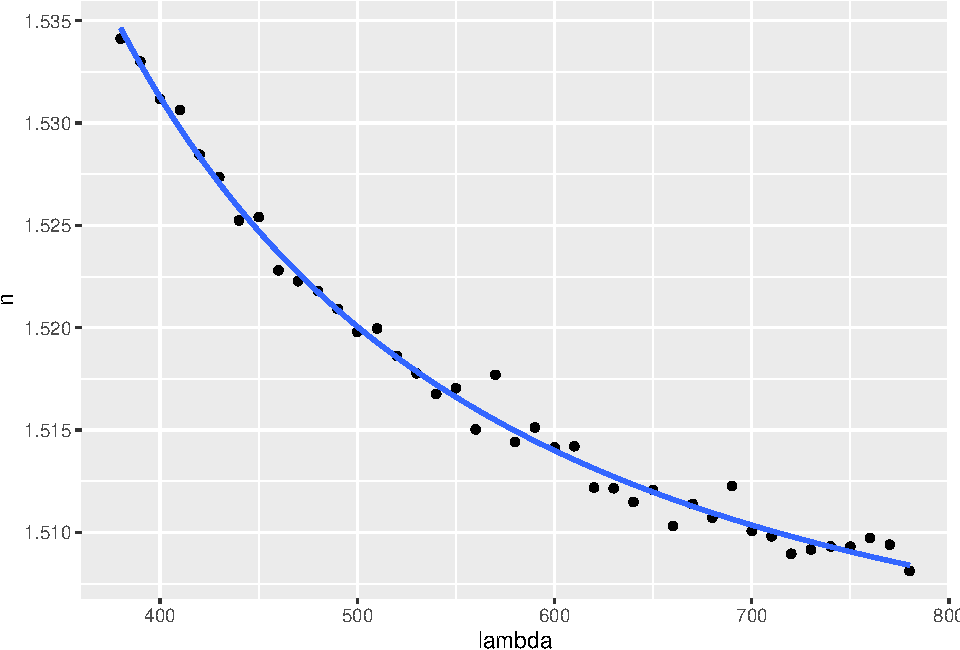
\includegraphics[width=1\linewidth]{Pr1-fitting_files/figure-latex/unnamed-chunk-19-1} \end{center}

En los argumentos de \texttt{geom\_smooth()} hemos escrito \texttt{method\ =\ "lm"} para indicar que el ajuste se realiza con la función \texttt{lm()}.

Notar que al especificar la fórmula del modelo en el argumento \texttt{formula} no se utilizan los nombres \texttt{lambda} y \texttt{n} de las variables (como se hizo en la función \texttt{lm()}) sino los nombres \texttt{x} e \texttt{y} de las estéticas asociadas.

El argumento \texttt{se\ =\ FALSE} inhibe representar los intervalos de confianza (que estudiaremos en el segundo bloque del curso).

\hypertarget{nls}{%
\section{Modelos no lineales}\label{nls}}

Modelos como
\[y = \beta_1 \beta_2^{x}\]
(modelo exponencial) o como
\[y = \beta_1x^{\beta_2}\]
(modelo potencial) no tienen una estructura lineal.

Para modelos lineales, el problema de encontrar los valores de los parámetros que minimizan el error cuadrático del ajuste se traduce en resolver el sistema de ecuaciones normales de Gauss, que es un sistema lineal.\\
Pero en el caso de modelos no lineales como los anteriores, la situación se complica porque ahora la solución viene dada por un sistema de ecuaciones no lineal.

En este capítulo veremos cómo ajustar este tipo de modelos a una colección de observaciones, usando la función \texttt{nls()} (\textbf{n}onlinea \textbf{l}east \textbf{s}quares) de \textsf{R}.

\hypertarget{planteamiento-del-problema-ley-de-enfriamiento-de-newton}{%
\subsection{Planteamiento del problema: Ley de enfriamiento de Newton}\label{planteamiento-del-problema-ley-de-enfriamiento-de-newton}}

La ley de enfriamiento de Newton establece que cuando un sólido a temperatura inicial \(T_0\) se deja enfriar en un ambiente de temperatura \(T_a\), su temperatura en función del tiempo \(t\) viene dada por
\[T(t)=T_a+(T_0-T_a)e^{-kt}\]
donde \(k\) es una constante que depende de la forma del sólido y del calor específico del material que lo componga.

En un experimento se calentó una barra de hierro hasta una temperatura inicial de \(T_0\) y después se dejó enfriar en un ambiente a temperatura \(T_a\). Se midió la temperatura de la barra a intervalos de tiempo de \(1\) minuto, durante una hora. Los datos obtenidos se recogen en el archivo \href{https://drive.google.com/uc?export=download\&id=1mpF0_lZVw-u2SlrxJDwczEI4x_OxO1W2}{\texttt{newton.csv}}(click para descargar), que contiene las variables:

\begin{itemize}
\item
  \texttt{time}: tiempo transcurrido, en minutos, desde el instante inicial (\(t=0\)).
\item
  \texttt{temp}: temperatura de la barra de hierro, en ºC.
\end{itemize}

Como antes, descarga el fichero \texttt{newton.csv} y guárdalo en una carpeta de nombre \texttt{data} dentro de tu directorio de trabajo. Importamos los datos con \texttt{read\_csv()} y los guardamos en un objeto de nombre \texttt{newton}:

\begin{Shaded}
\begin{Highlighting}[]
\NormalTok{newton }\OtherTok{\textless{}{-}} \FunctionTok{read\_csv}\NormalTok{(}\StringTok{"data/newton.csv"}\NormalTok{)}
\end{Highlighting}
\end{Shaded}

Visualizamos los datos dibujando la nube de puntos \((t, T)\) con \texttt{geom\_point()}:

\begin{Shaded}
\begin{Highlighting}[]
\FunctionTok{ggplot}\NormalTok{(}
    \AttributeTok{data =}\NormalTok{ newton,}
    \AttributeTok{mapping =} \FunctionTok{aes}\NormalTok{(}\AttributeTok{x =}\NormalTok{ time, }\AttributeTok{y =}\NormalTok{ temp)}
\NormalTok{) }\SpecialCharTok{+} 
    \FunctionTok{geom\_point}\NormalTok{()}
\end{Highlighting}
\end{Shaded}

\begin{center}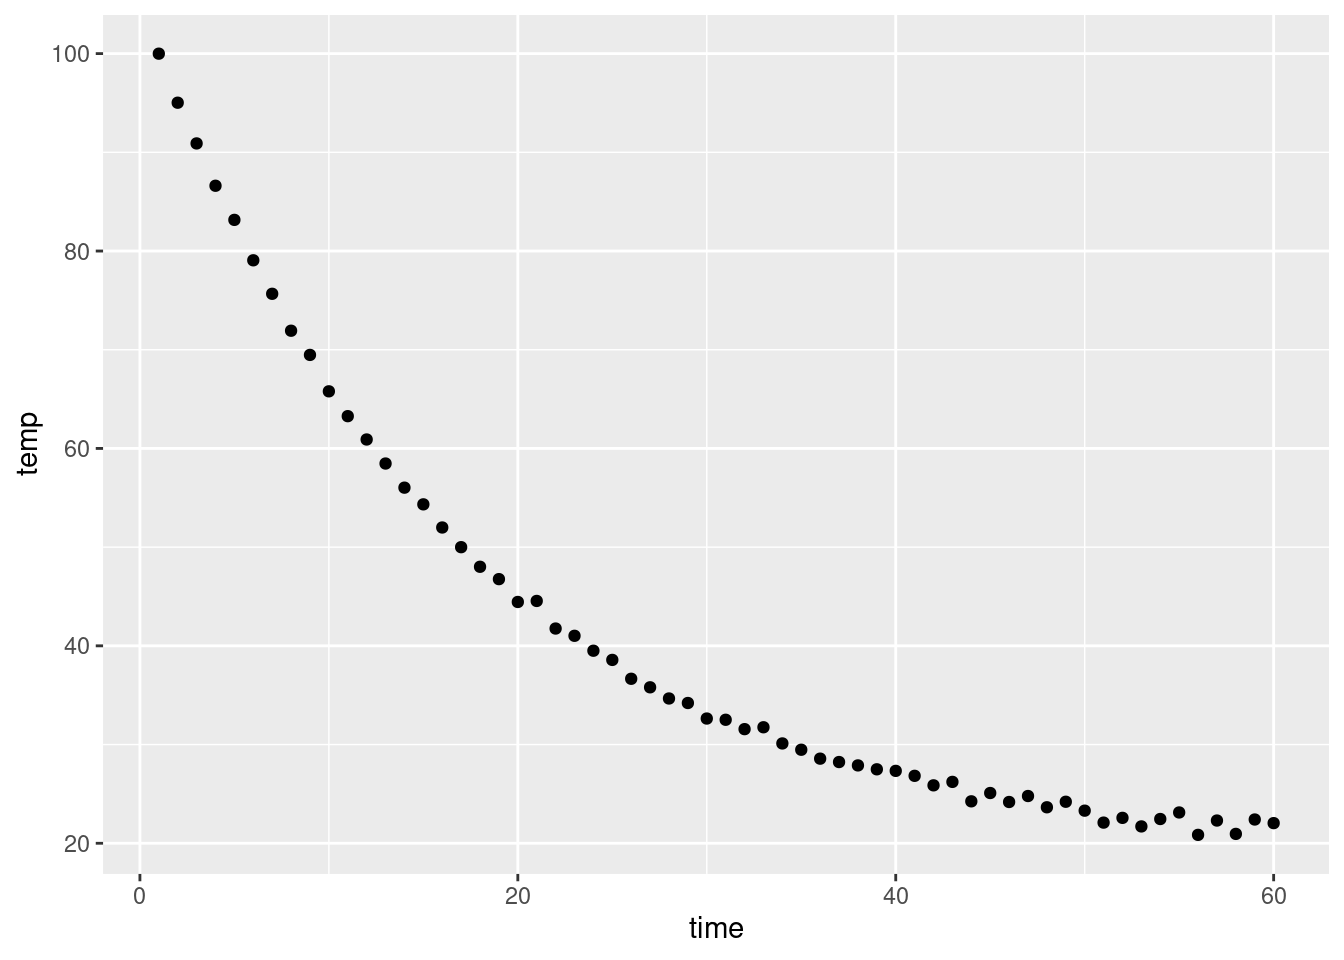
\includegraphics[width=1\linewidth]{Pr1-fitting_files/figure-latex/unnamed-chunk-23-1} \end{center}

\hypertarget{ajuste-con-nls}{%
\subsection{\texorpdfstring{Ajuste con \texttt{nls()}}{Ajuste con nls()}}\label{ajuste-con-nls}}

Antes de utilizar la función \texttt{nls()} necesitamos crear una función para la fórmula de la temperatura en nuestro modelo, que tiene como argumentos la variable independiente \(t\), y los tres parámetros \(T_0\), \(T_a\) y \(k\):

\begin{Shaded}
\begin{Highlighting}[]
\NormalTok{T\_model }\OtherTok{\textless{}{-}} \ControlFlowTok{function}\NormalTok{(t, Ta, T0, k)\{}
\NormalTok{    Ta }\SpecialCharTok{+}\NormalTok{ (T0}\SpecialCharTok{{-}}\NormalTok{Ta)}\SpecialCharTok{*}\FunctionTok{exp}\NormalTok{(}\SpecialCharTok{{-}}\NormalTok{k}\SpecialCharTok{*}\NormalTok{t)}
\NormalTok{\}}
\end{Highlighting}
\end{Shaded}

También necesitamos proporcionar unos valores iniciales para los parámetros. Estos valores iniciales ayudarán en el proceso de optimización del error cuadrático (que pasa por resolver un sistema no lineal). A la vista de los datos tomaremos \(20\) como valor inicial para \(T_a\) y \(100\) como valor inicial para \(T_0\). Para el valor inicial de \(k\), tomamos \(0.05\). (En la tarea de evaluación se propondrán los valores iniciales para los correspondientes parámetros).

Con los elementos anteriores, ya podemos utilizar la función \texttt{nls()}. Utilizaremos la función \texttt{T\_model} que acabamos de definir para el valor del argumento \texttt{formula}, e indicaremos los valores iniciales de los parámetros en el argumento \texttt{start}, en forma de lista con la función \texttt{list()}:

\begin{Shaded}
\begin{Highlighting}[]
\NormalTok{fit\_newton }\OtherTok{\textless{}{-}} \FunctionTok{nls}\NormalTok{(}
    \AttributeTok{data =}\NormalTok{ newton, }
    \AttributeTok{formula =}\NormalTok{ temp }\SpecialCharTok{\textasciitilde{}} \FunctionTok{T\_model}\NormalTok{(time, Ta, T0, k),}
    \AttributeTok{start =} \FunctionTok{list}\NormalTok{(}\AttributeTok{Ta =} \DecValTok{20}\NormalTok{, }\AttributeTok{T0 =} \DecValTok{100}\NormalTok{,  }\AttributeTok{k =} \FloatTok{0.05}\NormalTok{)}
\NormalTok{)}
\end{Highlighting}
\end{Shaded}

\hypertarget{coeficientes-1}{%
\subsection{Coeficientes}\label{coeficientes-1}}

Los coeficientes del ajuste son:

\begin{Shaded}
\begin{Highlighting}[]
\FunctionTok{coefficients}\NormalTok{(fit\_newton)}
\end{Highlighting}
\end{Shaded}

\begin{verbatim}
##           Ta           T0            k 
##  19.02958737 104.98070986   0.05994108
\end{verbatim}

Redondeando los resultados a dos decimales, las estimaciones obtenidas son
\[\hat{T_a} = 19.03,\]
\[\hat{T_0}=104.98,\]
y
\[\hat{k}=0.06,\]
y el ajuste quedaría:

\[T(t) = 19.03 + (104.98-19.03)e^{-0.06t}.\]

\hypertarget{predicciones-1}{%
\subsection{Predicciones}\label{predicciones-1}}

Los pronósticos para las temperaturas a la que se encontrará la barra de hierro a los \(70\), \(80\) y \(90\) minutos serían:

\begin{Shaded}
\begin{Highlighting}[]
\FunctionTok{predict}\NormalTok{(}
\NormalTok{    fit\_newton,}
    \FunctionTok{tibble}\NormalTok{(}\AttributeTok{time =} \FunctionTok{c}\NormalTok{(}\DecValTok{70}\NormalTok{, }\DecValTok{80}\NormalTok{, }\DecValTok{90}\NormalTok{))}
\NormalTok{)}
\end{Highlighting}
\end{Shaded}

\begin{verbatim}
## [1] 20.32380 19.74029 19.41986
\end{verbatim}

\hypertarget{gruxe1fico-ajuste}{%
\subsection{Gráfico ajuste}\label{gruxe1fico-ajuste}}

Como en el capítulo anterior usamos la función \texttt{geom\_smooth()} para representar el ajuste:

\begin{Shaded}
\begin{Highlighting}[]
\FunctionTok{ggplot}\NormalTok{(}
    \AttributeTok{data =}\NormalTok{ newton, }
    \AttributeTok{mapping =} \FunctionTok{aes}\NormalTok{(}\AttributeTok{x =}\NormalTok{ time, }\AttributeTok{y =}\NormalTok{ temp)}
\NormalTok{) }\SpecialCharTok{+} 
    \FunctionTok{geom\_point}\NormalTok{() }\SpecialCharTok{+} 
    \FunctionTok{geom\_smooth}\NormalTok{(}
        \AttributeTok{method =} \StringTok{"nls"}\NormalTok{,}
        \AttributeTok{formula =}\NormalTok{ y }\SpecialCharTok{\textasciitilde{}} \FunctionTok{T\_model}\NormalTok{(x, T0, Ta, k),}
        \AttributeTok{method.args =} \FunctionTok{list}\NormalTok{(}
            \AttributeTok{start =} \FunctionTok{list}\NormalTok{(}\AttributeTok{T0 =} \DecValTok{100}\NormalTok{, }\AttributeTok{Ta =} \DecValTok{20}\NormalTok{, }\AttributeTok{k =} \FloatTok{0.05}\NormalTok{)}
\NormalTok{        ),}
        \AttributeTok{se =} \ConstantTok{FALSE} \CommentTok{\# intervalo de confianza no implementado en predict.nls}
\NormalTok{    )}
\end{Highlighting}
\end{Shaded}

\begin{center}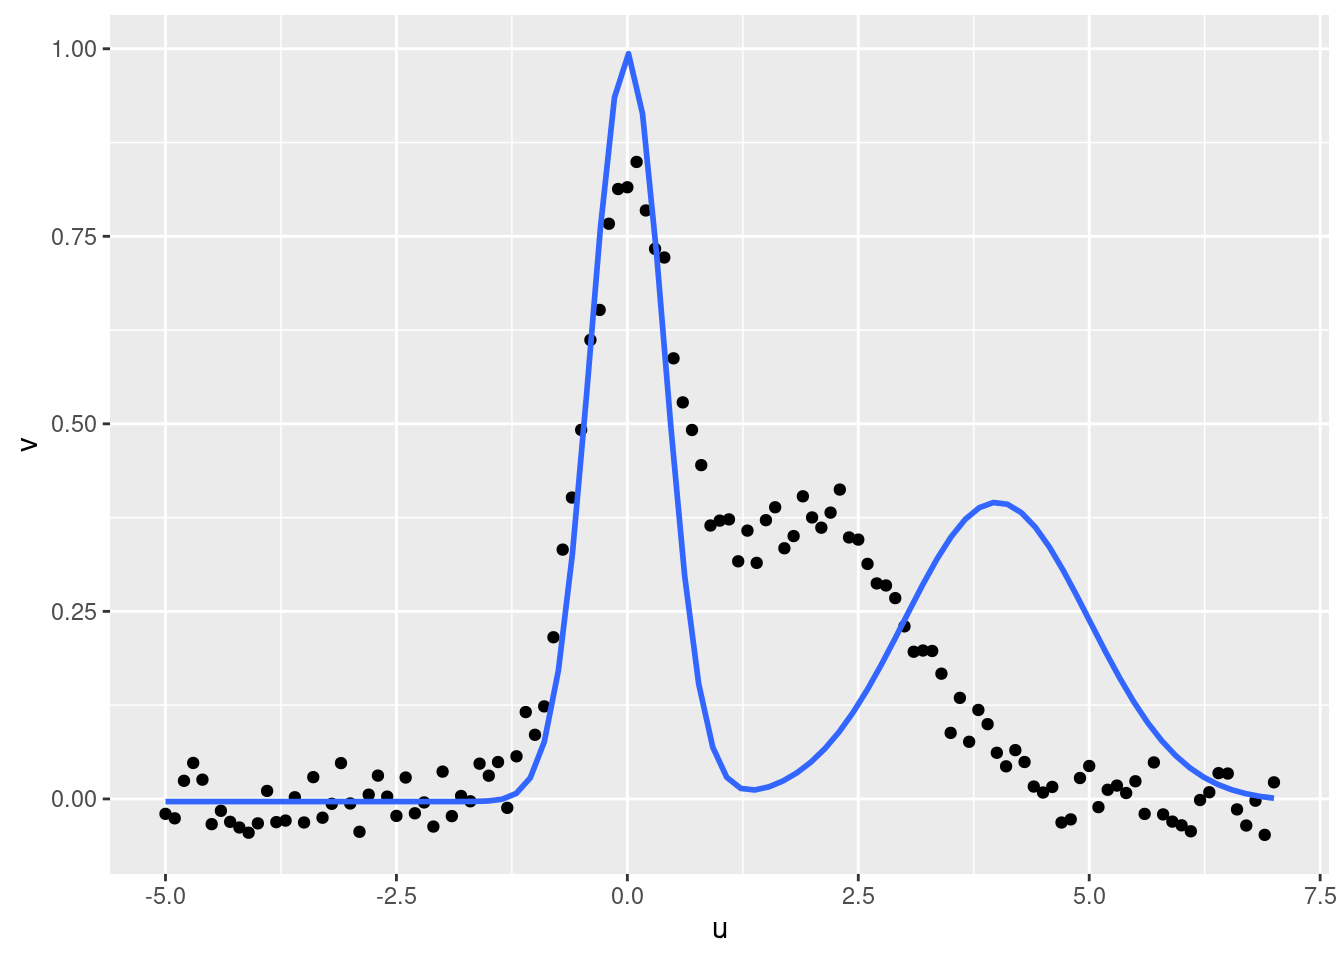
\includegraphics[width=1\linewidth]{Pr1-fitting_files/figure-latex/unnamed-chunk-28-1} \end{center}

En los argumentos de \texttt{geom\_smooth()} hemos escrito ahora \texttt{method\ =\ "nls"} para indicar que el ajuste se realiza con la función \texttt{nls()}.

El argumento \texttt{start} que requiere la función \texttt{nls()} se especifica en \texttt{method.args\ =\ list(...)}.

Notar que hemos usado nuestra función \texttt{T\_model()} para especificar la fórmula del modelo, como al usar la función \texttt{nls()}, pero que en este caso no se utilizan los nombres \texttt{time} y \texttt{temp} de las variables sino los nombres \texttt{x} e \texttt{y} de las correspondientes estéticas.

El argumento \texttt{se\ =\ FALSE} es necesario en este caso (si no lo incluyes obtendrás un error) por una cuestión técnica que no vamos a detallar.

% After Body

\end{document}
